% =====================================================================
%  CPE 333 Operating Systems 1/2569 - Problem Session 7
%  Concurrency and Thread
%  ---------------------------------------------------------------
%  คอมไพล์ด้วย XeLaTeX
% =====================================================================
\documentclass[a4paper,11pt]{article}

% ------------------------- Layout -------------------------
\usepackage[margin=2.2cm,top=2.2cm,bottom=2.2cm]{geometry}
\usepackage{fancyhdr}
\setlength{\headheight}{14pt}
\usepackage{parskip}
\setlength{\parskip}{4pt}
\usepackage{enumitem}
\setlist{topsep=3pt,itemsep=2pt,parsep=0pt}
\usepackage{booktabs}
\usepackage{graphicx}
\usepackage{float}
\usepackage{caption}
\captionsetup{font=small,skip=3pt}
\usepackage{xcolor}
\usepackage{listings}
\usepackage[hidelinks]{hyperref}

% ------------------------- ฟอนต์ภาษาไทย -------------------------
\usepackage{fontspec}
\usepackage{xltxtra}

\setmainfont{TH Sarabun New}[Scale=1.45]
\setmonofont{Consolas}[Scale=0.78]

% การตัดคำภาษาไทย
\XeTeXlinebreaklocale "th"
\XeTeXlinebreakskip = 0pt plus 0.3pt
\emergencystretch=3em

% ------------------------- สไตล์โค้ด -------------------------
\definecolor{codebg}{RGB}{248,248,248}
\definecolor{codeframe}{RGB}{221,221,221}
\definecolor{kw}{RGB}{0,86,179}
\definecolor{cmt}{RGB}{106,153,85}
\definecolor{str}{RGB}{163,21,21}
\definecolor{numgray}{RGB}{150,150,150}

\lstdefinestyle{cstyle}{
  language=C,
  backgroundcolor=\color{codebg},
  frame=single,
  rulecolor=\color{codeframe},
  basicstyle=\ttfamily\scriptsize,
  keywordstyle=\color{kw}\bfseries,
  commentstyle=\color{cmt}\itshape,
  stringstyle=\color{str},
  numbers=left,
  numberstyle=\tiny\color{numgray},
  numbersep=6pt,
  showstringspaces=false,
  breaklines=true,
  breakatwhitespace=true,
  tabsize=4,
  captionpos=b,
  aboveskip=6pt,
  belowskip=2pt,
  xleftmargin=12pt,
  framexleftmargin=12pt,
  morekeywords={pthread_t,pthread_create,pthread_join,sched_yield,taskset,objdump},
}

\lstdefinestyle{terminal}{
  language={},
  keywordstyle=\relax,
  commentstyle=\relax,
  stringstyle=\relax,
  backgroundcolor=\color{codebg},
  frame=single,
  rulecolor=\color{codeframe},
  basicstyle=\ttfamily\scriptsize,
  numbers=none,
  breaklines=true,
  showstringspaces=false,
  captionpos=b,
  aboveskip=6pt,
  belowskip=2pt,
  xleftmargin=4pt,
}

\lstset{style=cstyle}
\renewcommand{\lstlistingname}{Code}
\newcommand{\code}[1]{\texttt{#1}}

% ------------------------- Header / Footer -------------------------
\pagestyle{fancy}
\fancyhf{}
\lhead{\small CPE 333 Operating Systems 1/2569}
\rhead{\small Problem Session 7}
\cfoot{\thepage}
\renewcommand{\headrulewidth}{0.4pt}


% =====================================================================
\begin{document}

% ------------------------- หน้าปก -------------------------
\begin{titlepage}
\centering
\vspace*{0.3cm}

\includegraphics[width=3.2cm]{KMUTT_CI_Primary_Logo-Full-1200x1200.png}\\[0.8cm]
{\Large\bfseries รายงานปฏิบัติการ}\\[0.4cm]
{\Large\bfseries PS07: Concurrency and Thread}\\[0.4cm]
\vfill
{\large\bfseries เสนอ}\\[0.3cm]
{\large อาจารย์ ราชวิชช์ สโรชวิกสิต}\\[1.2cm]
{\large\bfseries จัดทำโดย}\\[0.4cm]
\renewcommand{\arraystretch}{1.35}
\begin{tabular}{l@{\hspace{1.5cm}}l}
นายภูมิพัฒน์ อภิวาทธนะพงศ์ & 67070501035 \\
นายวิรชัช ทองอุทัยศรี & 67070501041 \\
นายเจษฎา เกียรติกมลวงศ์ & 67070501080 \\
\end{tabular}
\renewcommand{\arraystretch}{1.0}
\vfill
{\large รายงานนี้เป็นส่วนหนึ่งของวิชา CPE 333 Operating Systems}\\[0.2cm]
{\large ภาควิชาวิศวกรรมคอมพิวเตอร์ คณะวิศวกรรมศาสตร์}\\[0.2cm]
{\large ภาคการศึกษาที่ 1 ปีการศึกษา 2569}\\[0.2cm]
{\large มหาวิทยาลัยเทคโนโลยีพระจอมเกล้าธนบุรี}
\end{titlepage}

% หน้าปกและสารบัญไม่นับเลขหน้า เนื้อหาจริงเริ่มนับที่หน้า 1
\thispagestyle{empty}
\tableofcontents
\newpage
\setcounter{page}{1}

% =====================================================================
\section*{สภาพแวดล้อมที่ใช้ในการทดลอง}
\addcontentsline{toc}{section}{สภาพแวดล้อมที่ใช้ในการทดลอง}
% =====================================================================

การทดลองทั้งหมดทำบน Linux ที่ทำงานอยู่บน WSL2 ของเครื่องคอมพิวเตอร์เครื่องเดียว จุดที่มีผลต่อการทดลองนี้โดยตรงคือจำนวน CPU เพราะ thread ที่รันบน CPU คนละแกนทำงานพร้อมกันได้จริง ไม่ต้องรอให้ระบบปฏิบัติการสลับให้ รายละเอียดของสภาพแวดล้อมเป็นดังนี้

\begin{table}[H]
\centering\small
\caption{ข้อมูลสภาพแวดล้อมของระบบที่ใช้ในการทดลอง}
\begin{tabular}{@{}p{3.9cm}p{12.2cm}@{}}
\toprule
\textbf{รายการ} & \textbf{รายละเอียด} \\
\midrule
ระบบปฏิบัติการ & Ubuntu 24.04.1 LTS ทำงานบน WSL2 ของ Windows 11 Home Single Language (build 26200) \\
Kernel & \code{6.6.87.2-microsoft-standard-WSL2} (x86-64, \code{SMP PREEMPT\_DYNAMIC}) \\
CPU & Intel Core Ultra 9 185H ที่ Linux มองเห็นเป็น 22 logical CPU (11 core แกนละ 2 thread) \\
คอมไพเลอร์ & \code{gcc 13.3.0} ไม่ระบุระดับ optimization จึงใช้ค่าเริ่มต้นคือ \code{-O0} \\
Thread library & POSIX threads ของ \code{glibc 2.39} (ลิงก์ด้วย \code{-lpthread}) \\
เครื่องมือเสริม & \code{taskset} (util-linux) สำหรับบังคับให้ process ทำงานบน CPU ที่กำหนด \\
\bottomrule
\end{tabular}
\end{table}

\textbf{หมายเหตุเรื่องหลักฐาน:} ผลการรันทุกครั้งที่แสดงในรายงานเป็นภาพหน้าจอจริงจาก terminal ตัวเลขทุกตัวที่อ้างถึงในคำอธิบายและในตารางสรุปอ่านมาจากภาพโดยตรง ภาพทั้งหมดเก็บไว้ที่ \code{PS07/result/screenshots/} และลำดับคำสั่งที่ใช้ถ่ายภาพอยู่ใน \code{PS07/docs/COMMANDS.md}

% =====================================================================
\section{ภาพรวมของโปรแกรม}
% =====================================================================

\subsection{สถานการณ์ที่เลือก: บัญชีเงินฝากร่วมที่ใช้ผ่านตู้ ATM หลายตู้พร้อมกัน}

ตัวอย่างในคาบเรียนใช้ thread หลายตัวบวกค่าตัวนับ (counter) ตัวเดียวกันไปในทิศทางเดียว รายงานนี้เลือกสถานการณ์ที่ต่างออกไปคือ \textbf{บัญชีเงินฝากร่วมหนึ่งบัญชี} ที่มีตู้ ATM หลายตู้ทำรายการพร้อมกัน โดยแต่ละตู้คือ thread หนึ่งตัว และยอดเงินในบัญชีคือตัวแปรที่ทุก thread ใช้ร่วมกัน

\begin{itemize}[leftmargin=*]
  \item บัญชีเปิดด้วยยอดเงิน 1,000 บาท (\code{INITIAL\_BALANCE})
  \item thread ครึ่งแรกเป็น \textbf{ตู้ฝากเงิน} ฝากครั้งละ 1 บาท ส่วน thread ครึ่งหลังเป็น \textbf{ตู้ถอนเงิน} ถอนครั้งละ 1 บาท ทุก thread ทำรายการเท่ากันคือ \code{tx} ครั้ง
  \item เงินที่ไหลเข้าจึงเท่ากับเงินที่ไหลออกเสมอ \textbf{ยอดเงินสุดท้ายที่ถูกต้องต้องเท่ากับ 1,000 บาท} ไม่ว่าจะใช้กี่ thread และไม่ว่าจะทำรายการกี่ครั้ง
\end{itemize}

สถานการณ์นี้ต่างจากตัวอย่างในคาบเรียนสามข้อ ข้อแรกคือมีการเปลี่ยนค่า\textbf{สองทิศทาง} (ทั้งเพิ่มและลด) ตามที่ใบงานกำหนดให้มีทั้ง increase และ decrease ผลของ race condition จึงออกมาได้ทั้งเป็นบวกและเป็นลบ ข้อที่สองคือความผิดพลาดมีความหมายชัดเจน ถ้ายอดสุดท้ายสูงกว่า 1,000 บาทแปลว่ารายการถอนบางรายการหายไป (ธนาคารเสียเงิน) ถ้าต่ำกว่าแปลว่ารายการฝากบางรายการหายไป (ลูกค้าเสียเงิน) และข้อที่สามคือโปรแกรม\textbf{ตรวจสอบตัวเอง}ได้ เพราะแต่ละ thread นับจำนวนรายการที่ตัวเองทำเสร็จไว้ในตัวแปร local ที่ไม่มีใครใช้ร่วม จึงพิสูจน์ได้ว่ารายการทุกรายการถูกทำจริงครบถ้วน สิ่งที่ผิดมีแต่ยอดเงินในตัวแปรที่ใช้ร่วมกันเท่านั้น

\subsection{โครงสร้างของโปรแกรม}

ตัวแปรที่ทุก thread ใช้ร่วมกันมีเพียงตัวเดียวคือ \code{balance} ซึ่งเป็นตัวแปร global จึงอยู่ในส่วน data ของ process และทุก thread ใน process เดียวกันมองเห็นตำแหน่งหน่วยความจำเดียวกัน ส่วนข้อมูลของแต่ละตู้เก็บใน \code{struct atm} หนึ่งชุดต่อหนึ่ง thread

\begin{lstlisting}[caption={ตัวแปรที่ใช้ร่วมกันและข้อมูลประจำตัวของแต่ละ thread}]
#define INITIAL_BALANCE 1000L
#define AMOUNT          1L
#define MAX_THREADS     64

long balance = INITIAL_BALANCE;

int use_yield = 0;              /* set once in main() before any thread starts */

enum role { DEPOSITOR, WITHDRAWER, BOTH };

struct atm {
    pthread_t tid;
    enum role role;
    long      tx;               /* transactions this thread must make     */
    long      deposits;         /* written once by the thread when done:  */
    long      withdrawals;      /* how many transactions it really made   */
};
\end{lstlisting}

การฝากและถอนเขียนเป็นฟังก์ชันสั้น ๆ ที่แก้ค่า \code{balance} ตรง ๆ โดยไม่มี lock หรือกลไก synchronization ใด ๆ ป้องกันไว้ ซึ่งเป็นจุดที่ใบงานกำหนดให้มี (\textit{without proper synchronization})

\begin{lstlisting}[caption={การฝากและถอนเงินที่ไม่มีการป้องกัน}]
void deposit_plain(void)
{
    balance = balance + AMOUNT;
}

void withdraw_plain(void)
{
    balance = balance - AMOUNT;
}
\end{lstlisting}

ฟังก์ชันที่ทุก thread รันคือ \code{atm\_thread()} ซึ่งวนทำรายการตามบทบาทของตัวเอง ตัวนับ \code{done\_dep} และ \code{done\_wdr} เป็นตัวแปร local ที่อยู่บน stack ของแต่ละ thread แยกกัน จึงไม่มีทางเกิด race condition และค่าที่นับได้ถูกต้องเสมอ thread เขียนค่าเหล่านี้กลับเข้า \code{struct atm} ของตัวเองเพียงครั้งเดียวตอนทำงานเสร็จ ส่วน pointer to function สองตัวแรก (\code{deposit} และ \code{withdraw}) เลือกว่าจะใช้ฟังก์ชันฝาก--ถอนแบบใด ใน Task 1 และ Task 2 จะเป็น \code{deposit\_plain()} และ \code{withdraw\_plain()} เสมอ ส่วนแบบ \code{\_yield} ใช้ใน Task 3

\begin{lstlisting}[caption={ฟังก์ชันที่แต่ละ thread รัน}]
void *atm_thread(void *arg)
{
    struct atm *a = arg;
    void (*deposit)(void)  = use_yield ? deposit_yield  : deposit_plain;
    void (*withdraw)(void) = use_yield ? withdraw_yield : withdraw_plain;
    long done_dep = 0, done_wdr = 0;
    long i;

    if (a->role == DEPOSITOR || a->role == BOTH)
        for (i = 0; i < a->tx; i++) {
            deposit();
            done_dep++;
        }
    if (a->role == WITHDRAWER || a->role == BOTH)
        for (i = 0; i < a->tx; i++) {
            withdraw();
            done_wdr++;
        }

    a->deposits    = done_dep;
    a->withdrawals = done_wdr;
    return NULL;
}
\end{lstlisting}

ฟังก์ชัน \code{main()} รับค่าจาก command line ในรูป \code{./ps7 [threads] [tx\_per\_thread] [yield]} ตัวแรกคือจำนวน thread ตัวที่สองคือจำนวนรายการต่อ thread (ค่าเริ่มต้นคือ 1 thread และ 1,000,000 รายการ คำสั่ง \code{./ps7} เฉย ๆ ตามใบงานจึงใช้ได้) และตัวที่สามซึ่งไม่บังคับคือคำว่า \code{yield} สำหรับ Task 3 ตัวแปร \code{use\_yield} ถูกตั้งค่าเพียงครั้งเดียวก่อนสร้าง thread หลังจากนั้นทุก thread อ่านอย่างเดียว จึงไม่เกิด race condition กับตัวแปรนี้ จากนั้นกำหนดบทบาทของแต่ละ thread ตามตารางด้านล่าง สร้าง thread ทั้งหมดด้วย \code{pthread\_create()} ก่อนแล้วจึงรอทุกตัวด้วย \code{pthread\_join()} เพื่อให้ทุก thread ทำงานซ้อนกันได้ สุดท้ายรวมจำนวนรายการจากทุก thread มาคำนวณยอดที่ควรจะเป็น (\code{expected}) แล้วเทียบกับยอดจริง (\code{actual})

\begin{table}[H]
\centering\small
\caption{บทบาทของ thread ตามจำนวน thread ที่ระบุ}
\begin{tabular}{@{}p{3.2cm}p{12.9cm}@{}}
\toprule
\textbf{จำนวน thread} & \textbf{บทบาท} \\
\midrule
1 & thread เดียวฝากเงิน \code{tx} ครั้งแล้วจึงถอน \code{tx} ครั้ง ใช้เป็นผลอ้างอิงแบบทำทีละรายการตามลำดับ (Task 1) \\
เลขคู่ตั้งแต่ 2 ถึง 64 & thread ครึ่งแรกฝากเงินอย่างเดียว ครึ่งหลังถอนเงินอย่างเดียว แต่ละตัวทำ \code{tx} รายการ (Task 2 และ Task 3) \\
เลขคี่ที่มากกว่า 1 & ไม่รับ เพราะแบ่งฝากกับถอนให้เท่ากันไม่ได้ โปรแกรมพิมพ์วิธีใช้แล้วจบการทำงาน \\
\bottomrule
\end{tabular}
\end{table}

แต่ละรอบการรันพิมพ์ผลเพียงบรรทัดเดียว เพื่อให้ภาพหน้าจอหนึ่งภาพแสดงผลของการรันซ้ำได้หลายรอบ ความหมายของแต่ละช่องเป็นดังนี้

\begin{lstlisting}[style=terminal,caption={รูปแบบผลลัพธ์หนึ่งบรรทัดต่อการรันหนึ่งรอบ}]
[plain] threads=4 tx=1000000 in=2000000 out=2000000 | expected=1000 actual=... diff=... RACE
\end{lstlisting}

\begin{itemize}[leftmargin=*]
  \item \code{[plain]} หรือ \code{[yield]} บอกว่ารอบนั้นใช้ฟังก์ชันฝาก--ถอนแบบใด
  \item \code{threads} และ \code{tx} คือจำนวน thread และจำนวนรายการต่อ thread ที่ระบุตอนรัน
  \item \code{in} และ \code{out} คือจำนวนรายการฝากและถอนทั้งหมดที่ thread นับได้จริง (จากตัวนับ local)
  \item \code{expected} คือยอดที่ควรเป็น คำนวณจาก \code{1000 + in - out} ซึ่งเท่ากับ 1,000 เสมอ
  \item \code{actual} คือค่าใน \code{balance} หลังทุก thread ทำงานเสร็จ และ \code{diff} คือ \code{actual - expected}
  \item คำสุดท้ายเป็น \code{OK} เมื่อ \code{diff} เท่ากับศูนย์ และเป็น \code{RACE} เมื่อยอดเงินผิด
\end{itemize}

\subsection{การคอมไพล์}

คอมไพล์ด้วยคำสั่งตามใบงานทุกตัวอักษร คือ \code{gcc -o ps7 ps7.c -lpthread} ตัวเลือก \code{-lpthread} บอก linker ให้ลิงก์กับ POSIX thread library ส่วนการที่\textbf{ไม่ระบุระดับ optimization} (จึงเป็น \code{-O0}) เป็นความตั้งใจ เพราะถ้าใช้ \code{-O2} คอมไพเลอร์มีสิทธิ์มองว่าลูปที่บวก \code{balance} ทีละ 1 เป็นล้านครั้งมีผลเท่ากับการบวกครั้งเดียว และรวบทั้งลูปเหลือคำสั่งเดียว ช่วงเวลาที่ thread สองตัวจะชนกันจึงแทบหายไป ทั้งที่โค้ดยังผิดอยู่เหมือนเดิม

% =====================================================================
\section{Task 1: รันด้วย thread เดียว}
% =====================================================================

ใบงานข้อ 2 ให้รันโปรแกรมด้วย thread เดียวก่อน เพื่อยืนยันว่าตรรกะของโปรแกรมถูกต้อง ถ้าผลที่ได้ในขั้นนี้ผิด ความผิดพลาดในขั้นต่อไปก็จะแยกไม่ออกว่าเกิดจาก race condition หรือเกิดจาก bug ธรรมดาในโปรแกรม

\subsection{การคอมไพล์และสภาพแวดล้อม}

\begin{figure}[H]
\centering
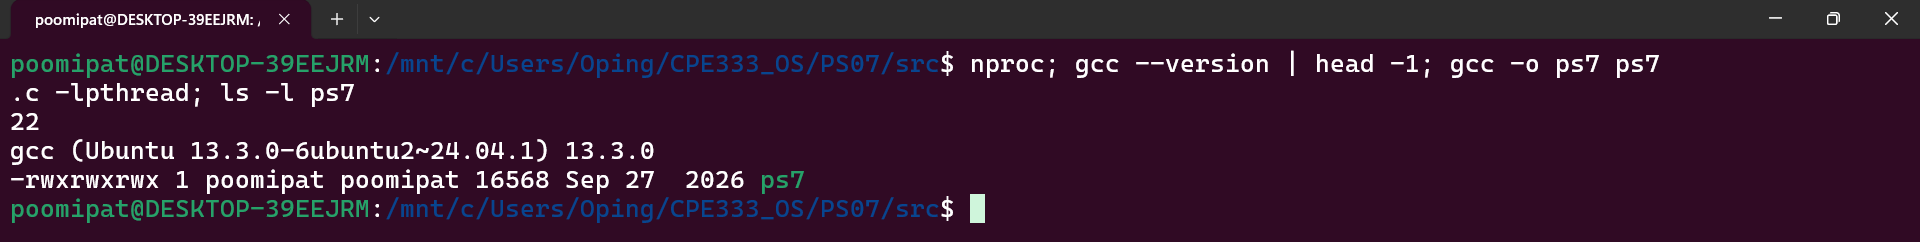
\includegraphics[width=\textwidth]{../result/screenshots/t01_env_compile.png}
\caption{จำนวน CPU รุ่นของ gcc และการคอมไพล์ด้วยคำสั่งตามใบงาน}
\end{figure}

จากภาพ คำสั่ง \code{nproc} ตอบ \code{22} คือ Linux มองเห็น CPU 22 ตัว ซึ่งหมายความว่า thread หลายตัวของโปรแกรมนี้ได้ CPU คนละตัวและทำงานพร้อมกันได้จริง ข้อนี้จะมีผลมากใน Task 2 คอมไพเลอร์คือ \code{gcc 13.3.0} ของ Ubuntu คำสั่ง \code{gcc -o ps7 ps7.c -lpthread} ไม่พิมพ์ข้อความใดออกมาเลย แปลว่าคอมไพล์ผ่านโดยไม่มีทั้ง error และ warning และ \code{ls -l} แสดงไฟล์ \code{ps7} ขนาด 16,568 byte ที่มีสิทธิ์ execute (สิทธิ์ขึ้นเป็น \code{rwxrwxrwx} ทุกช่อง เพราะไฟล์อยู่บน drive C ของ Windows ที่ WSL2 mount ไว้ที่ \code{/mnt/c})

\subsection{ผลการรันด้วย thread เดียว}

\begin{figure}[H]
\centering
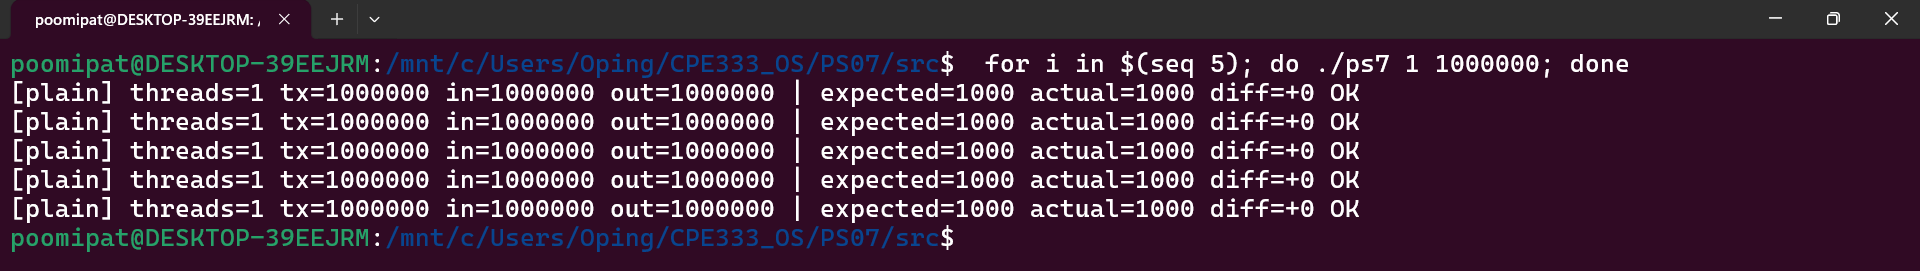
\includegraphics[width=\textwidth]{../result/screenshots/t02_task1_one_thread.png}
\caption{Task 1: รันด้วย thread เดียว 5 รอบ ได้ยอดเงินถูกต้องทุกรอบ}
\end{figure}

คำสั่ง \code{./ps7 1 1000000} สร้าง thread ทำงานเพียงตัวเดียว (thread \code{main} มีหน้าที่แค่สร้างแล้วรอด้วย \code{pthread\_join()} และไม่แตะ \code{balance} จนกว่า thread ทำงานจะจบ) thread ตัวนี้ฝากเงิน 1,000,000 ครั้งจนยอดขึ้นไปเป็น 1,001,000 บาท แล้วจึงถอนอีก 1,000,000 ครั้งจนยอดกลับลงมา

ผลทั้ง 5 รอบในภาพเหมือนกันทุกตัวอักษร คือ \code{in=1000000 out=1000000 | expected=1000 actual=1000 diff=+0 OK} แสดงว่า
\begin{itemize}[leftmargin=*]
  \item ตรรกะของโปรแกรมถูกต้อง ทั้งการกำหนดบทบาท การวนทำรายการ ตัวนับ local และการคำนวณยอดที่ควรเป็น
  \item ผลลัพธ์ \textbf{deterministic} คือรันกี่ครั้งก็ได้ค่าเดิม เพราะมี thread เพียงตัวเดียวที่อ่านและเขียน \code{balance} การอ่าน--บวก--เขียนแต่ละครั้งจึงจบครบก่อนเริ่มครั้งถัดไปเสมอ
  \item แม้ระบบปฏิบัติการจะขัดจังหวะ thread ตัวนี้กลางคันเพื่อไปรันงานอื่นได้ตลอดเวลา แต่ค่าที่ค้างอยู่ใน register ถูกเก็บไว้กับ context ของ thread และถูกคืนกลับมาครบเมื่อได้ทำงานต่อ และระหว่างนั้นไม่มี thread อื่นแก้ \code{balance} ค่าที่เขียนกลับจึงยังถูกต้อง
\end{itemize}

ผลนี้เป็นเส้นฐานสำหรับเทียบกับขั้นต่อไป ถ้าใช้หลาย thread แล้วยอดเงินผิดไปจาก 1,000 บาท สาเหตุจึงไม่ใช่ bug ในตรรกะของโปรแกรม แต่มาจากการที่หลาย thread แก้ตัวแปรเดียวกันพร้อมกันเท่านั้น

% =====================================================================
\section{Task 2: หลาย thread โดยไม่บังคับ context switch}
% =====================================================================

ใบงานข้อ 3 ให้แก้โปรแกรมให้สร้าง thread มากกว่าหนึ่งตัว และข้อ 4 ให้รันโดยไม่บังคับ context switch หลาย ๆ ครั้งเพื่อดูว่าผลไม่แน่นอน โปรแกรมนี้รับจำนวน thread จาก command line อยู่แล้ว การแก้ในขั้นนี้จึงเป็นการสั่ง \code{./ps7 4 1000000} แทน \code{./ps7 1 1000000} ซึ่งทำให้ \code{main()} สร้าง thread 4 ตัว เป็นตู้ฝากเงิน 2 ตัวและตู้ถอนเงิน 2 ตัว แต่ละตัวทำ 1,000,000 รายการ รวมเป็นฝาก 2,000,000 ครั้งและถอน 2,000,000 ครั้ง ยอดที่ถูกต้องจึงยังเป็น 1,000 บาทเหมือนเดิม ตัวฟังก์ชัน \code{deposit\_plain()} และ \code{withdraw\_plain()} ไม่ได้แก้เลยแม้แต่บรรทัดเดียว

การทดลองนี้รันสองแบบ แบบแรกปล่อยให้ระบบปฏิบัติการจัดวาง thread บน CPU ทั้ง 22 ตัวตามปกติ แบบที่สองใช้ \code{taskset -c 0} บังคับให้ทุก thread อยู่บน CPU หมายเลข 0 ตัวเดียว เพื่อแยกให้เห็นว่าผลที่ผิดเกิดจากกลไกใด

\subsection{รันบน CPU 22 ตัว}

\begin{figure}[H]
\centering
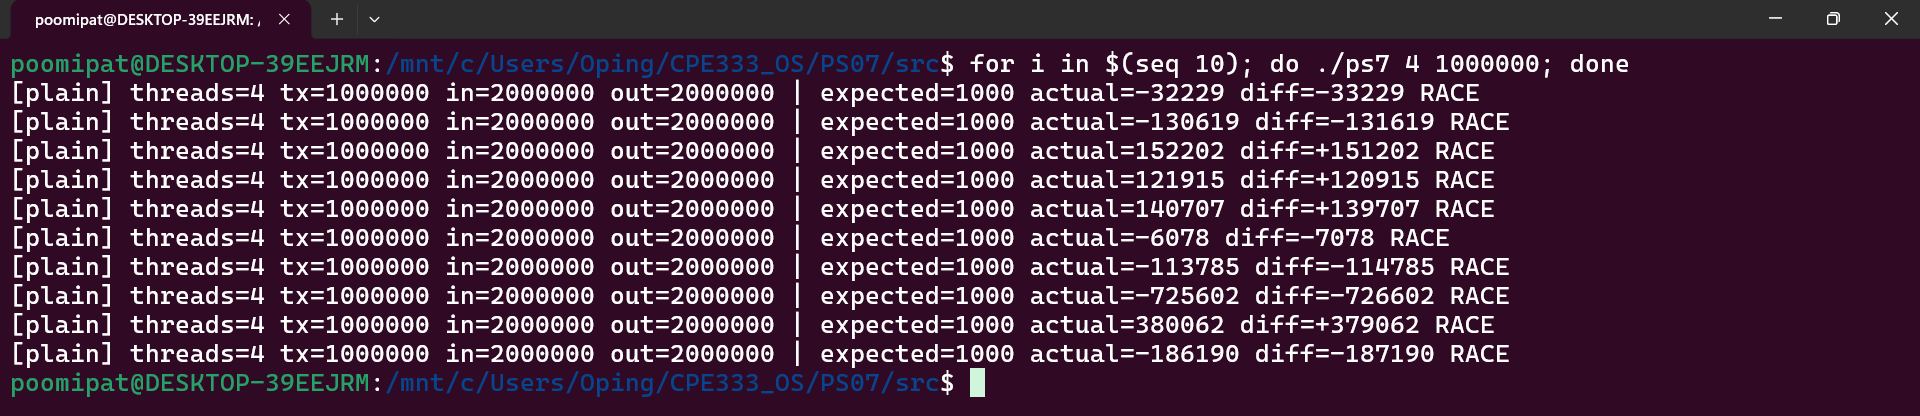
\includegraphics[width=\textwidth]{../result/screenshots/t03_task2_multicore.png}
\caption{Task 2: 4 thread บน CPU 22 ตัว รัน 10 รอบ ผิดทุกรอบและไม่ซ้ำกันเลย}
\end{figure}

ทั้ง 10 รอบในภาพลงท้ายด้วย \code{RACE} ค่า \code{diff} ของแต่ละรอบเรียงตามลำดับคือ \mbox{-33,229}, \mbox{-131,619}, +151,202, +120,915, +139,707, \mbox{-7,078}, \mbox{-114,785}, \mbox{-726,602}, +379,062 และ \mbox{-187,190} ข้อสังเกตจากภาพมีดังนี้

\begin{itemize}[leftmargin=*]
  \item \textbf{ผลไม่ซ้ำกันเลยสักรอบ} ทั้งที่เป็นโปรแกรมเดียวกัน รับ argument เดียวกัน และรันบนเครื่องเดียวกันติดต่อกัน นี่คือพฤติกรรมแบบ non-deterministic ที่ใบงานต้องการให้แสดง
  \item \textbf{ผิดได้ทั้งสองทิศทาง} มีรอบที่ยอดเกิน 4 รอบ (รายการถอนหายไปมากกว่ารายการฝาก ธนาคารเสียเงิน) และรอบที่ยอดขาด 6 รอบ (รายการฝากหายไปมากกว่า ลูกค้าเสียเงิน) รอบที่ผิดมากที่สุดยอดเงินขาดไป 726,602 บาท และรอบที่ใกล้เคียงที่สุดก็ยังผิด 7,078 บาท
  \item \textbf{รายการครบทุกรายการ} ช่อง \code{in=2000000 out=2000000} เท่ากันทุกบรรทัด แปลว่าทุก thread ทำรายการครบตามจำนวนจริง สิ่งที่หายไปคือ\textit{ผลของการเขียน}ลงตัวแปร \code{balance} ไม่ใช่ตัวรายการ
  \item ค่า \code{diff} เป็นเพียง\textbf{ผลสุทธิ}ระหว่างรายการฝากที่หายกับรายการถอนที่หาย ซึ่งหักล้างกันได้ จำนวนรายการที่หายไปจริงจึงมากกว่าหรือเท่ากับค่าสัมบูรณ์ของ \code{diff} เสมอ
\end{itemize}

สาเหตุที่ผิดทุกรอบในกรณีนี้คือเครื่องมี CPU มากพอให้ thread ทั้ง 4 ตัวได้ CPU คนละตัว thread จึง\textbf{ทำงานพร้อมกันจริง} (parallelism) ไม่ต้องรอให้ระบบปฏิบัติการสลับให้ ในทุก ๆ รอบของลูป CPU สองตัวมีโอกาสอ่านค่า \code{balance} ค่าเดียวกันไปพร้อมกัน แล้วต่างคนต่างเขียนผลของตัวเองกลับ ผลของตัวที่เขียนก่อนจึงถูกเขียนทับหายไป เมื่อลูปวนเป็นล้านรอบ การชนแบบนี้จึงเกิดขึ้นเป็นจำนวนมหาศาล และจำนวนที่ชนในแต่ละรอบการรันขึ้นอยู่กับจังหวะเวลาที่ควบคุมไม่ได้ เช่น thread ไหนเริ่มก่อน ได้ CPU ตัวใด และ CPU ตัวอื่นกำลังทำอะไรอยู่

\subsection{รันบน CPU ตัวเดียวด้วย taskset}

\begin{figure}[H]
\centering
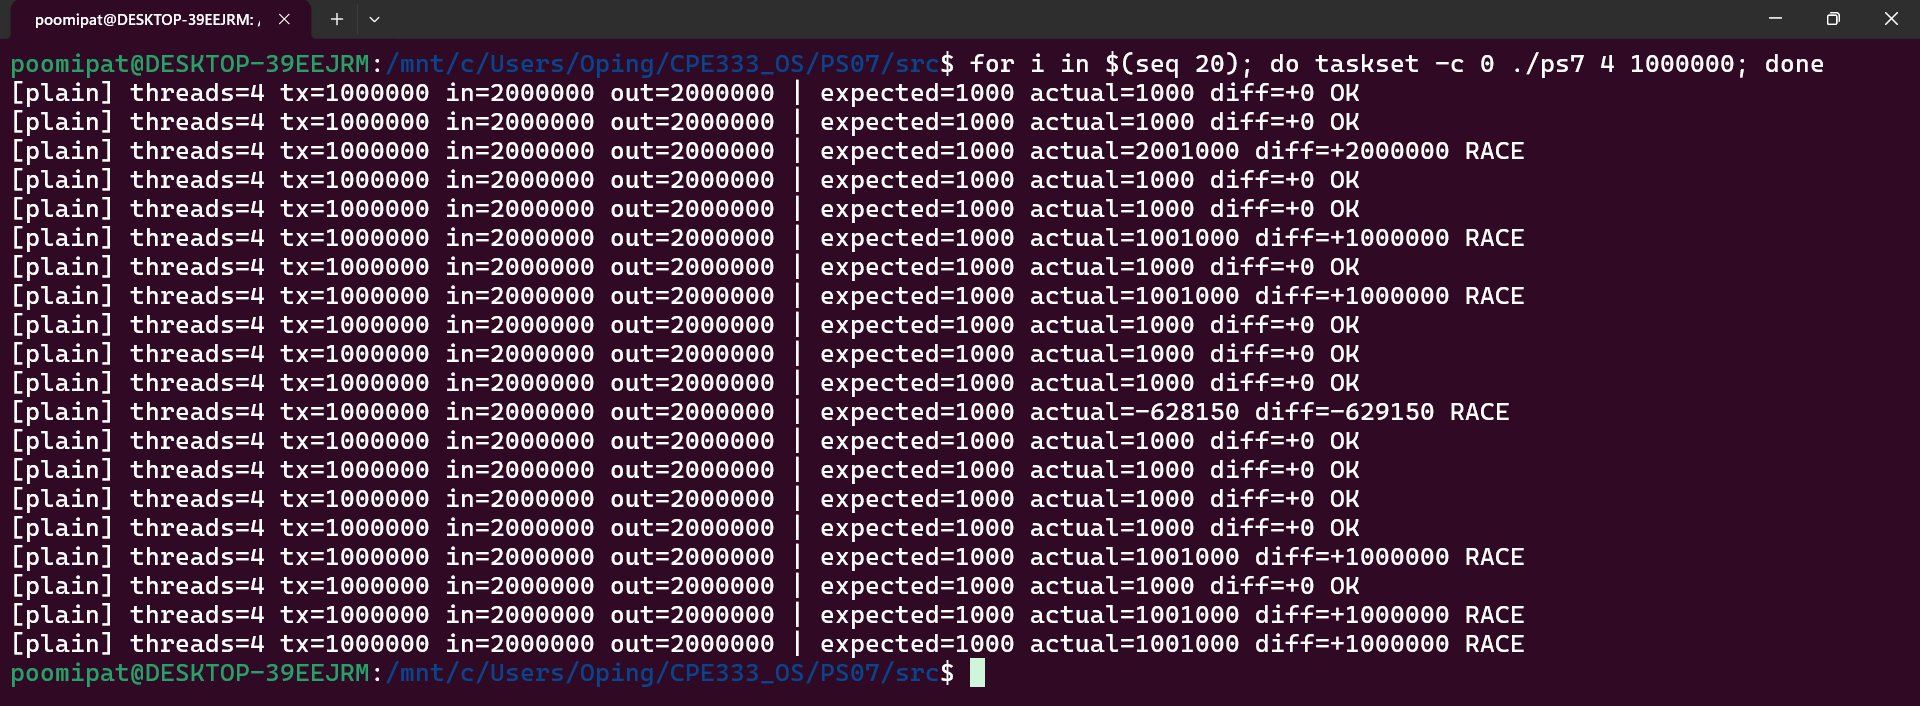
\includegraphics[width=\textwidth]{../result/screenshots/t04_task2_one_core.png}
\caption{Task 2: 4 thread บน CPU ตัวเดียว รัน 20 รอบ ถูก 13 รอบ ผิด 7 รอบ}
\end{figure}

เมื่อบังคับให้ทุก thread อยู่บน CPU ตัวเดียว ในแต่ละขณะจะมี thread ทำงานได้เพียงตัวเดียว thread จะสลับกันก็ต่อเมื่อ kernel ขัดจังหวะ thread ที่กำลังทำงาน (timer interrupt เมื่อหมด time slice) แล้วเลือก thread อื่นขึ้นมาทำงานแทน ผลในภาพต่างจากกรณี CPU 22 ตัวอย่างชัดเจน

\begin{itemize}[leftmargin=*]
  \item \textbf{ถูก 13 รอบ ผิด 7 รอบ} รอบที่ผิดคือรอบที่ 3, 6, 8, 12, 17, 19 และ 20 ส่วนที่เหลือได้ \code{actual=1000 diff=+0 OK}
  \item \textbf{เมื่อผิดจะผิดเป็นก้อนใหญ่ที่ลงตัว} รอบที่ 6, 8, 17, 19 และ 20 ได้ \code{diff=+1000000} พอดี ซึ่งเท่ากับงานทั้งหมดของ thread ถอนเงินหนึ่งตัว รอบที่ 3 ได้ \code{diff=+2000000} เท่ากับงานของ thread ถอนเงินทั้งสองตัว และรอบที่ 12 ได้ \code{diff=-629150} คือรายการฝาก 629,150 รายการหายไป
\end{itemize}

รูปแบบนี้อธิบายได้ด้วยจังหวะของ context switch ลูปของ thread หนึ่งตัว (1,000,000 รอบ) ใช้เวลาเพียงไม่กี่มิลลิวินาที thread ส่วนใหญ่จึงทำงานจบได้ในไม่กี่ time slice และถึงจะโดนขัดจังหวะ จุดที่โดนขัดก็มักไม่ตกอยู่ระหว่างการอ่านกับการเขียน \code{balance} รอบส่วนใหญ่จึงถูกต้อง แต่ถ้าบังเอิญ thread ฝากเงินตัวหนึ่งโดนขัดจังหวะ\textbf{หลังจากอ่านค่า \code{balance} เข้า register แล้วแต่ยังไม่ได้เขียนกลับ} ค่าใน register นั้นจะถูกเก็บไว้กับ context ของมัน ระหว่างที่รอ thread ถอนเงินได้ขึ้นมาทำงานและถอนครบทั้ง 1,000,000 ครั้ง เมื่อ thread ฝากเงินได้กลับมาทำงานต่อ มันเขียนค่าเก่าที่ค้างอยู่ทับลงไป รายการถอนทั้งล้านรายการจึงหายไปในการเขียนครั้งเดียว ได้ \code{diff=+1000000} พอดี กรณี \code{diff=-629150} ก็เป็นกลไกเดียวกันในทิศตรงข้าม คือ thread ถอนเงินถือค่าเก่าค้างไว้ขณะที่ thread ฝากเงินทำไปได้ 629,150 รายการ

นี่คือ \textbf{untimely context switch} ตามที่ใบงานอธิบาย ซึ่งเกิดขึ้นได้เองตามธรรมชาติแต่ไม่บ่อย จึงต้องรันหลายครั้งถึงจะเห็น และเป็นเหตุผลที่ Task 3 ต้องบังคับให้เกิด

\subsection{ทำไม \code{balance = balance + AMOUNT} จึงไม่ปลอดภัย}

คำสั่ง C หนึ่งบรรทัดดูเหมือนทำงานเสร็จในขั้นเดียว แต่ CPU ไม่ได้บวกค่าในหน่วยความจำโดยตรง ภาพด้านล่างใช้ \code{objdump} แปลงไฟล์ \code{ps7} ตัวเดียวกับที่ใช้รันใน t03 และ t04 กลับเป็นภาษา assembly (รูปแบบ Intel ที่เขียนปลายทางไว้ก่อนต้นทาง)

\begin{figure}[H]
\centering
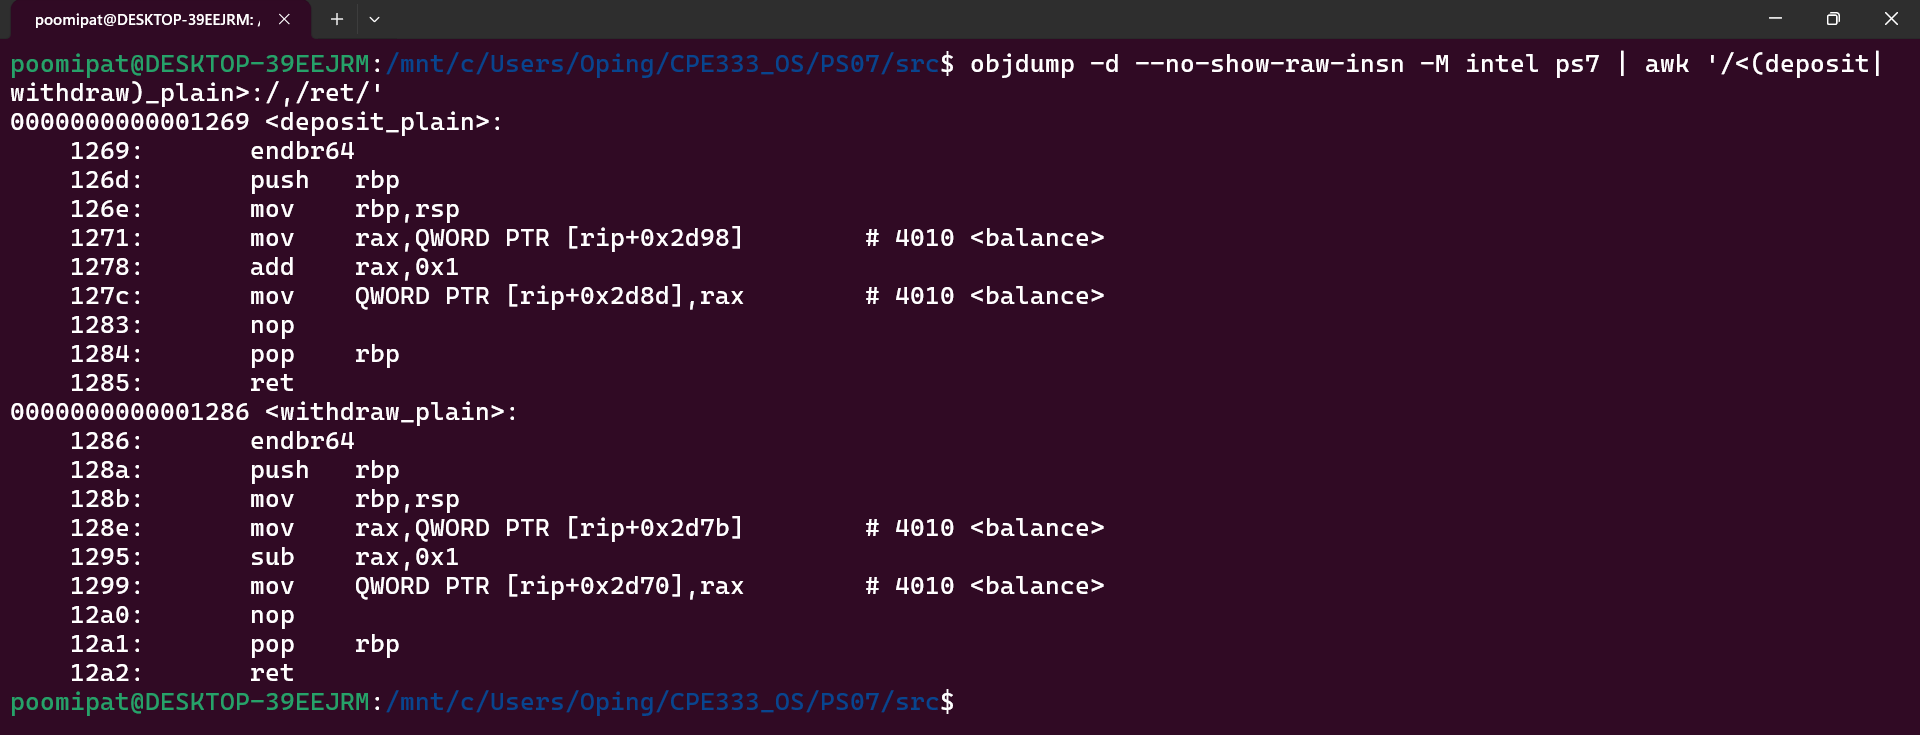
\includegraphics[width=0.85\textwidth]{../result/screenshots/t05_objdump.png}
\caption{คำสั่งเครื่องของ \code{deposit\_plain()} และ \code{withdraw\_plain()}}
\end{figure}

ทั้งสองฟังก์ชันมีโครงเหมือนกัน คำสั่งที่เหลือเป็นเพียงการเข้าและออกจากฟังก์ชัน ส่วนที่เป็นหัวใจของ race condition คือสามคำสั่งตรงกลาง ซึ่ง \code{objdump} ระบุไว้ท้ายบรรทัดว่าอ้างถึงตัวแปร \code{<balance>} ที่ตำแหน่ง \code{4010} เดียวกัน

\begin{table}[H]
\centering\small
\caption{สามขั้นของการแก้ค่า \code{balance} ที่อ่านได้จากภาพ}
\begin{tabular}{@{}p{1.5cm}p{2.4cm}p{4.3cm}p{7.0cm}@{}}
\toprule
\textbf{ขั้น} & \textbf{ที่อยู่} & \textbf{คำสั่ง} & \textbf{ความหมาย} \\
\midrule
Load & \code{1271} / \code{128e} & \code{mov rax,QWORD PTR [...]} & อ่านค่า \code{balance} จากหน่วยความจำมาไว้ใน register \code{rax} \\
Modify & \code{1278} / \code{1295} & \code{add rax,0x1} / \code{sub rax,0x1} & บวกหรือลบ 1 เฉพาะใน register หน่วยความจำยังเป็นค่าเดิม \\
Store & \code{127c} / \code{1299} & \code{mov QWORD PTR [...],rax} & เขียนค่าใน \code{rax} กลับลง \code{balance} ทับค่าที่อยู่ในหน่วยความจำขณะนั้น \\
\bottomrule
\end{tabular}
\end{table}

ปัญหาอยู่ที่ช่วงเวลาระหว่าง Load กับ Store ถ้ามี thread อื่นแก้ \code{balance} ในช่วงนี้ ไม่ว่าจะเพราะทำงานพร้อมกันบน CPU อีกตัว (t03) หรือเพราะ thread นี้ถูกสลับออกไปกลางคัน (t04) ขั้น Store จะเขียนค่าที่คำนวณจากข้อมูลเก่าทับลงไป และการแก้ของ thread อื่นจะหายไปโดยไม่มีสัญญาณเตือนใด ๆ การอ่าน--แก้--เขียน (read-modify-write) สามขั้นนี้จึง\textbf{ไม่เป็น atomic} และโค้ดส่วนนี้คือ critical section ที่ไม่มีการป้องกัน

\subsection{เปรียบเทียบผลบน CPU 22 ตัวกับ CPU ตัวเดียว}

\begin{table}[H]
\centering\small
\caption{เปรียบเทียบผลของ Task 2 ทั้งสองแบบ (อ่านจากภาพ t03 และ t04)}
\begin{tabular}{@{}p{2.8cm}p{6.4cm}p{6.4cm}@{}}
\toprule
\textbf{ประเด็น} & \textbf{CPU 22 ตัว (t03)} & \textbf{CPU ตัวเดียว (t04)} \\
\midrule
จำนวนรอบที่ผิด & 10 จาก 10 รอบ & 7 จาก 20 รอบ \\
ลักษณะของค่าที่ผิด & ไม่ซ้ำกันเลย มีทั้งบวกและลบ ตั้งแต่ \mbox{-726,602} ถึง +379,062 & ลงตัวเป็นก้อน ได้แก่ +1,000,000 จำนวน 5 รอบ, +2,000,000 และ \mbox{-629,150} อย่างละ 1 รอบ \\
ลักษณะการทำงาน & พร้อมกันจริงบน CPU คนละตัว & ทีละตัว สลับกันเมื่อ kernel ขัดจังหวะ \\
การชนเกิดเมื่อใด & ได้ทุกรอบของลูป เมื่อ CPU สองตัวเข้าช่วง Load--Store พร้อมกัน & เฉพาะเมื่อ context switch ตกระหว่าง Load กับ Store พอดี \\
\bottomrule
\end{tabular}
\end{table}

ทั้งสองแบบใช้โปรแกรมเดียวกันและผิดด้วยสาเหตุเดียวกัน คือการอ่าน--แก้--เขียนตัวแปรที่ใช้ร่วมกันโดยไม่มีการป้องกัน ต่างกันเพียงว่าอะไรเป็นตัวแทรกเข้ามาในช่วง Load--Store บนเครื่องที่มี CPU หลายตัว การทำงานพร้อมกันจริงทำให้ race condition ปรากฏแทบทุกครั้ง ส่วนบน CPU ตัวเดียว race condition จะปรากฏเฉพาะเมื่อ context switch เกิดขึ้นผิดจังหวะ ซึ่งเป็นเหตุการณ์ที่สุ่มและไม่บ่อย โปรแกรมที่มี bug แบบนี้จึงอาจผ่านการทดสอบหลายครั้งแล้วค่อยพังในภายหลัง

% =====================================================================
\section{Task 3: บังคับ context switch ระหว่างการอ่านกับการเขียน}
% =====================================================================

\subsection{การแก้โปรแกรม}

ใบงานข้อ 5 ให้เขียนโปรแกรมที่บังคับให้เกิด context switch ขณะกำลังแก้ค่าตัวแปร โดยแยกคำสั่ง \code{counter = counter + 1} ออกเป็นการอ่านค่าเข้า register การบวก และการเขียนกลับ แล้วเรียก \code{yield()} คั่นก่อนการเขียน โปรแกรมนี้จึงเพิ่มฟังก์ชันฝาก--ถอนอีกคู่หนึ่งที่เขียนสามขั้นนี้แยกกันให้เห็นชัดตามตัวอย่างในใบงาน

\begin{lstlisting}[caption={การฝากและถอนเงินที่บังคับ context switch ระหว่าง load กับ store}]
void deposit_yield(void)
{
    long reg = balance;         /* load   */
    reg = reg + AMOUNT;         /* modify */
    sched_yield();              /* force a context switch */
    balance = reg;              /* store  */
}

void withdraw_yield(void)
{
    long reg = balance;
    reg = reg - AMOUNT;
    sched_yield();
    balance = reg;
}
\end{lstlisting}

ตัวแปร local \code{reg} ทำหน้าที่แทน register ในตัวอย่างของใบงาน ค่าที่อ่านมาจึงค้างอยู่กับ thread นั้นในช่วงที่มันไม่ได้ทำงาน ส่วนฟังก์ชันที่ใช้บังคับสลับคือ \code{sched\_yield()} จาก \code{<sched.h>} ซึ่งเป็น system call มาตรฐานของ POSIX ที่บอก kernel ว่า thread นี้ยอมสละ CPU และขอไปต่อท้ายคิวของ thread ที่พร้อมทำงาน ไม่ได้ใช้ \code{pthread\_yield()} เพราะ glibc ตั้งแต่รุ่น 2.34 ประกาศเลิกใช้ฟังก์ชันนี้แล้ว และคอมไพเลอร์จะเตือนทุกครั้งที่เรียก

โหมดนี้เปิดด้วย argument ตัวที่สาม \code{yield} ซึ่งตั้งค่า \code{use\_yield} ให้ \code{atm\_thread()} เลือกใช้ฟังก์ชันคู่นี้แทนคู่เดิม ส่วนอื่นของโปรแกรมเหมือนเดิมทุกอย่าง จำนวนรายการต่อ thread ลดเหลือ 100,000 เพราะ \code{sched\_yield()} เป็น system call ที่ต้องเข้า kernel ทุกรอบของลูป จึงช้ากว่าการบวกเลขใน register หลายร้อยเท่า

\subsection{รันบน CPU 22 ตัว}

\begin{figure}[H]
\centering
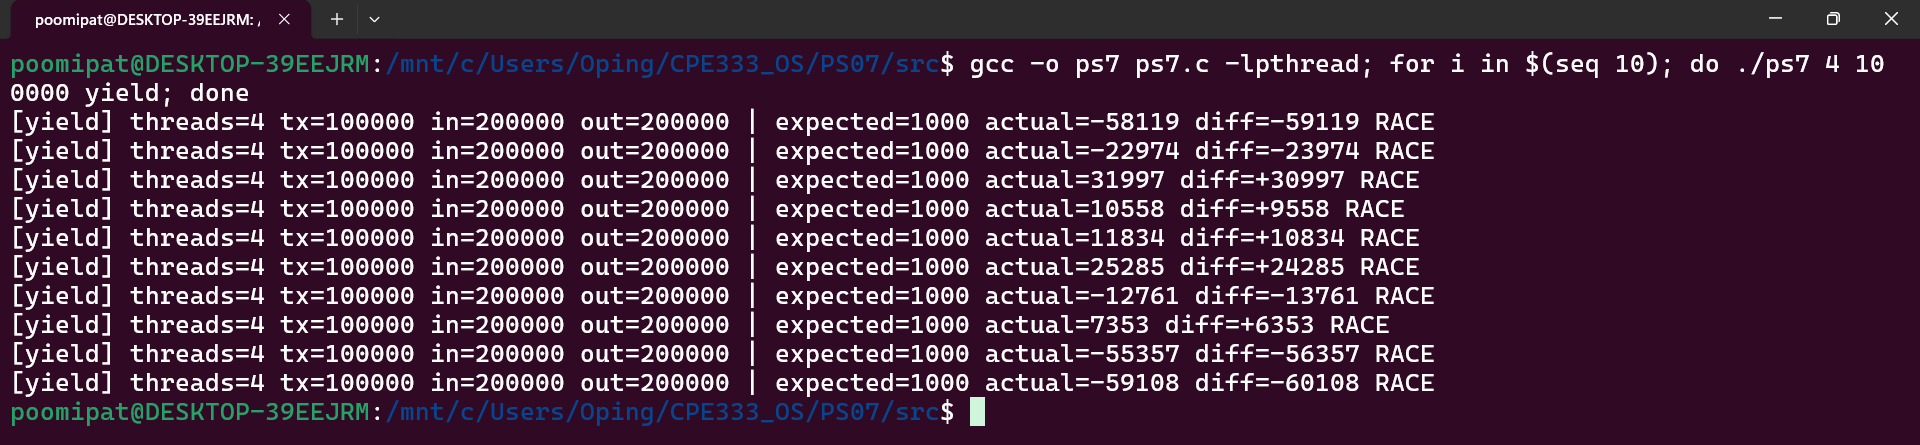
\includegraphics[width=\textwidth]{../result/screenshots/t06_task3_yield_multicore.png}
\caption{Task 3: คอมไพล์ใหม่แล้วรันโหมด yield บน CPU 22 ตัว 10 รอบ ผิดทุกรอบ}
\end{figure}

คอมไพล์ใหม่ด้วยคำสั่งเดิมผ่านโดยไม่มีข้อความใด ๆ จากนั้นรันโหมด yield 10 รอบ ทุกบรรทัดขึ้นต้นด้วย \code{[yield]} และลงท้ายด้วย \code{RACE} ค่า \code{diff} ของแต่ละรอบเรียงตามลำดับคือ \mbox{-59,119}, \mbox{-23,974}, +30,997, +9,558, +10,834, +24,285, \mbox{-13,761}, +6,353, \mbox{-56,357} และ \mbox{-60,108} เป็นบวก 5 รอบและลบ 5 รอบ ไม่ซ้ำกันเลยสักรอบ รอบที่ใกล้เคียงที่สุดก็ยังผิดไป 6,353 บาท ขณะที่ \code{in=200000 out=200000} เท่ากันทุกบรรทัดเช่นเคย

บนเครื่องที่มี CPU มากกว่าจำนวน thread แต่ละ thread มักได้ CPU ของตัวเอง เมื่อเรียก \code{sched\_yield()} แล้วไม่มี thread อื่นรออยู่บน CPU นั้น kernel จะให้ thread เดิมทำงานต่อทันทีโดยไม่สลับจริง (ตามที่ \code{sched\_yield(2)} ระบุ) ผลของ \code{sched\_yield()} ในกรณีนี้จึงเป็นการ\textbf{ยืดช่วงเวลาระหว่าง load กับ store} ให้ยาวขึ้นเป็นระยะเวลาของ system call หนึ่งครั้ง thread บน CPU อื่นจึงมีเวลาเขียน \code{balance} แทรกเข้ามาในช่วงนั้นได้มาก ผลจึงผิดทุกรอบเหมือน Task 2 แต่ race condition บน CPU หลายตัวเกิดขึ้นได้อยู่แล้วแม้ไม่มี yield ภาพนี้จึงยังไม่ได้แยกให้เห็นผลของการบังคับสลับโดยตรง การทดลองถัดไปทำหน้าที่นั้น

\subsection{รันบน CPU ตัวเดียว: เทียบโหมดปกติกับโหมด yield}

การทดลองนี้เป็นการทดลองแบบควบคุม คือรันบน CPU หมายเลข 0 ตัวเดียวด้วย \code{taskset -c 0} ใช้ 4 thread และ 100,000 รายการต่อ thread เท่ากันทุกรอบ รอบที่ 1--10 ใช้โหมดปกติ รอบที่ 11--20 ใช้โหมด yield สิ่งเดียวที่ต่างกันคือมีการเรียก \code{sched\_yield()} ระหว่าง load กับ store หรือไม่

\begin{figure}[H]
\centering
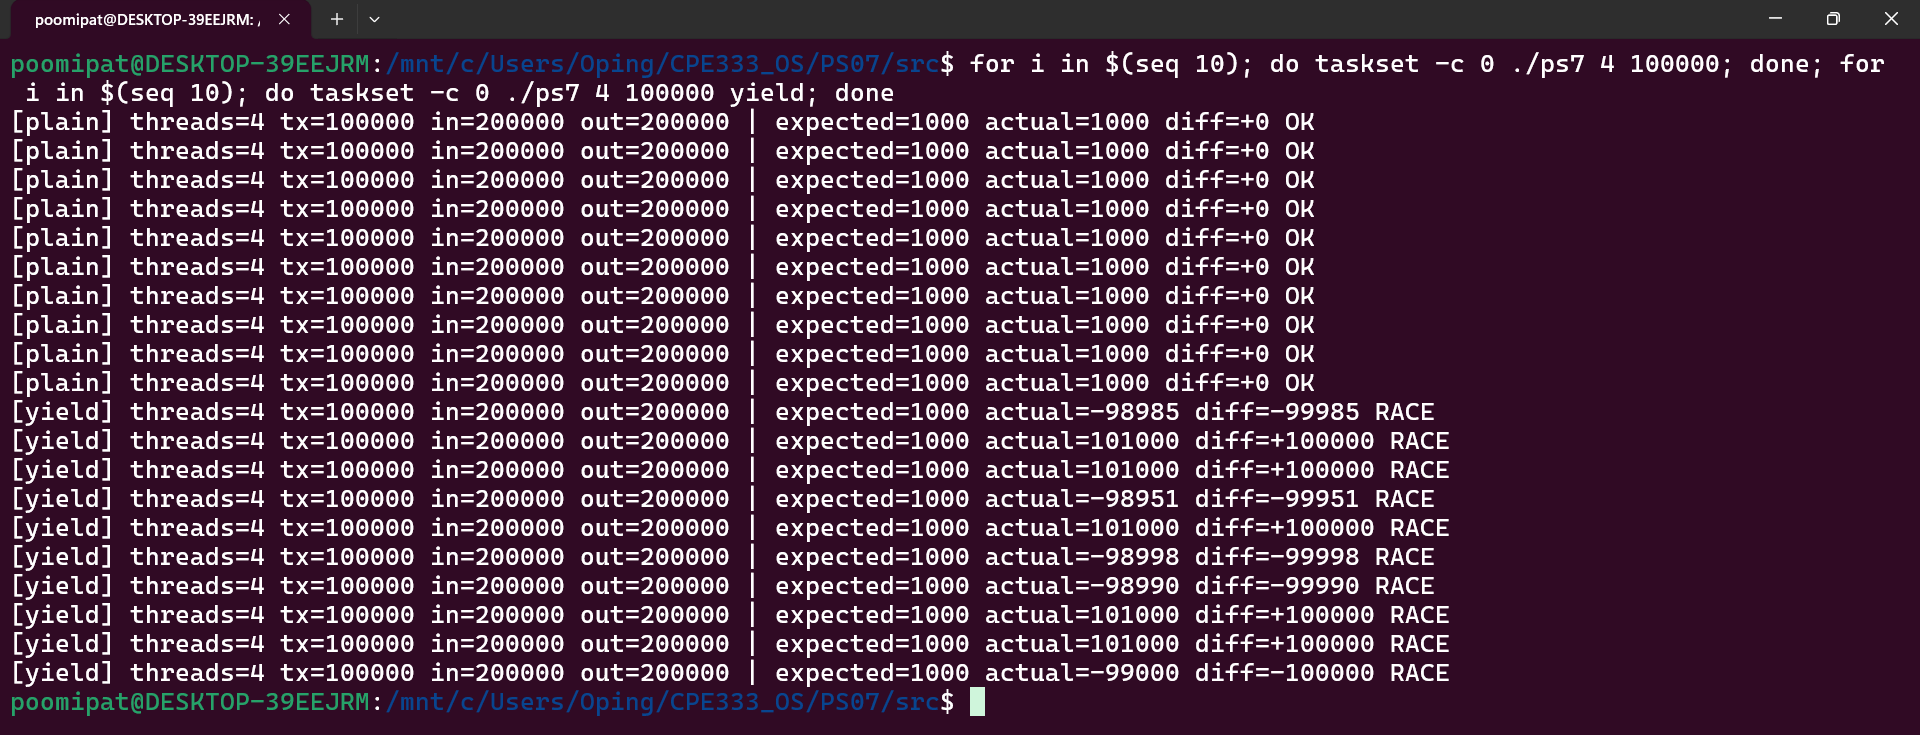
\includegraphics[width=\textwidth]{../result/screenshots/t07_task3_yield_one_core.png}
\caption{Task 3: CPU ตัวเดียว 100,000 รายการต่อ thread โหมดปกติถูกทั้ง 10 รอบ โหมด yield ผิดทั้ง 10 รอบ}
\end{figure}

\begin{itemize}[leftmargin=*]
  \item \textbf{โหมดปกติ 10 รอบแรกถูกทุกรอบ} (\code{actual=1000 diff=+0 OK}) เพราะลูป 100,000 รอบของแต่ละ thread สั้นมาก thread จึงมักทำงานจบก่อนหมด time slice และไม่ถูกขัดจังหวะระหว่าง load กับ store เลย
  \item \textbf{โหมด yield 10 รอบหลังผิดทุกรอบ} ค่า \code{diff} คือ \mbox{-99,985}, +100,000, +100,000, \mbox{-99,951}, +100,000, \mbox{-99,998}, \mbox{-99,990}, +100,000, +100,000 และ \mbox{-100,000} ได้ \code{+100000} พอดี 5 รอบ และอีก 5 รอบอยู่ใกล้ \code{-100000} มาก
\end{itemize}

ผลนี้ยืนยันว่า \textbf{context switch ที่เกิดผิดจังหวะคือตัวที่ทำให้เกิดการเขียนทับ} ในเมื่อโปรแกรมเดียวกันบน CPU ตัวเดียวกันถูกต้องทุกครั้งเมื่อไม่มี yield แต่ผิดทุกครั้งเมื่อบังคับให้สลับระหว่าง load กับ store

ส่วนเหตุที่ค่าผิดออกมาใกล้ +100,000 หรือ \mbox{-100,000} อธิบายได้ดังนี้ บน CPU ตัวเดียวที่มี 4 thread พร้อมทำงาน ทุกครั้งที่ thread เรียก \code{sched\_yield()} kernel จะสลับไปยัง thread ถัดไปในคิวจริง ๆ thread ทั้ง 4 ตัวจึงผลัดกันทำงานทีละหนึ่งรายการ ในแต่ละรอบ thread หนึ่งตัวจะ store ค่าที่ค้างไว้จากรอบก่อน แล้ว load ค่าที่ตัวเองเพิ่งเขียนนั้นกลับมาทันทีก่อนจะ yield อีกครั้ง ผลคือ thread ฝากเงินทั้งสองตัวเห็นแต่ค่าที่ฝั่งฝากเขียนไว้ และเดินขึ้นไปทีละ 1 ต่อรอบเหมือนเป็นตัวนับตัวเดียว (ฝาก 200,000 ครั้งแต่มีผลแค่ 100,000) ขณะที่ thread ถอนเงินทั้งสองตัวก็เดินลงทีละ 1 ต่อรอบในแบบเดียวกัน สองฝั่งนี้ต่างเขียนทับกันตลอดเวลา และยอดสุดท้ายคือค่าของฝั่งที่เขียนเป็นคนสุดท้าย ได้แก่ 1,000 + 100,000 = 101,000 ถ้าฝั่งฝากเขียนทีหลัง หรือ 1,000 - 100,000 = \mbox{-99,000} ถ้าฝั่งถอนเขียนทีหลัง ตรงกับ \code{actual=101000} และ \code{actual=-99000} ในภาพ ส่วนค่าที่คลาดจาก 100,000 ไปเล็กน้อย เช่น \mbox{-99,951} เกิดจากช่วงที่ลำดับการสลับไม่ได้เป็นระเบียบพอดี เช่น ตอนที่ thread เพิ่งถูกสร้างหรือเพิ่งทำงานจบ ฝั่งใดจะได้เขียนเป็นคนสุดท้ายขึ้นอยู่กับลำดับที่ scheduler จัดให้ในรอบนั้น ผลจึงสลับบวกและลบไปมาโดยคาดเดาไม่ได้

% =====================================================================
\section{อภิปรายผลและสาเหตุของ race condition}
% =====================================================================

\subsection{สาเหตุของ race condition ในโปรแกรมนี้}

race condition คือสถานการณ์ที่ผลลัพธ์ของโปรแกรมขึ้นอยู่กับลำดับหรือจังหวะเวลาที่ thread หลายตัวเข้าถึงข้อมูลเดียวกัน ในโปรแกรมนี้มีเงื่อนไขครบทั้งสามข้อที่ทำให้เกิด race condition

\begin{enumerate}[leftmargin=*]
  \item \textbf{มีข้อมูลที่ใช้ร่วมกัน} ตัวแปร global \code{balance} อยู่ในหน่วยความจำส่วนเดียวที่ทุก thread ของ process มองเห็น ต่างจาก \code{done\_dep} และ \code{done\_wdr} ที่อยู่บน stack ของแต่ละ thread แยกกัน ตัวนับเหล่านี้จึงถูกต้องเสมอ (\code{in} และ \code{out} ถูกทุกบรรทัดในทุกภาพ)
  \item \textbf{การแก้ค่าไม่เป็น atomic} คำสั่ง \code{balance = balance + AMOUNT} ถูกแปลเป็นสามคำสั่งเครื่องคือ load, add และ store (ภาพ t05) ระหว่างสามขั้นนี้ thread อื่นแทรกเข้ามาได้เสมอ
  \item \textbf{ไม่มีการกันไม่ให้เข้า critical section พร้อมกัน} (mutual exclusion) ไม่มี lock หรือกลไกใด ๆ บังคับให้ thread ทำสามขั้นนี้จบก่อนที่ thread อื่นจะเริ่ม
\end{enumerate}

ผลที่ตามมาเรียกว่า \textbf{lost update} คือการแก้ค่าของ thread หนึ่งถูกเขียนทับด้วยค่าที่อีก thread หนึ่งคำนวณจากข้อมูลเก่า ตารางด้านล่างแสดงลำดับเหตุการณ์ที่ทำให้รายการถอนเงินหนึ่งรายการหายไป ขั้นที่ 3--5 จะเกิดจาก thread B ทำงานพร้อมกันบน CPU อีกตัว (t03) หรือเกิดจาก thread A ถูกสลับออกหลังขั้นที่ 2 (t04 และ t07) ก็ได้ผลเหมือนกัน

\begin{table}[H]
\centering\small
\caption{ลำดับเหตุการณ์ที่ทำให้รายการถอนเงินหายไปหนึ่งรายการ}
\begin{tabular}{@{}p{1.2cm}p{4.9cm}p{4.9cm}p{4.0cm}@{}}
\toprule
\textbf{ลำดับ} & \textbf{thread A (ฝาก)} & \textbf{thread B (ถอน)} & \textbf{balance ในหน่วยความจำ} \\
\midrule
1 & load: \code{rax = 1000} & & 1000 \\
2 & add: \code{rax = 1001} & & 1000 \\
3 & & load: \code{rax = 1000} & 1000 \\
4 & & sub: \code{rax = 999} & 1000 \\
5 & & store: \code{balance = 999} & 999 \\
6 & store: \code{balance = 1001} & & 1001 \\
\bottomrule
\end{tabular}
\end{table}

ฝากหนึ่งครั้งและถอนหนึ่งครั้ง ยอดที่ถูกต้องต้องกลับมาเป็น 1,000 บาท แต่ได้ 1,001 บาทเพราะ thread A เขียนค่า 1001 ซึ่งคำนวณจากค่า 1000 ที่อ่านไว้ก่อน B จะถอน ทับผลของ B ไป ถ้าขั้นที่ 5 กับขั้นที่ 6 สลับลำดับกัน ยอดจะเป็น 999 บาทแทน คือรายการฝากของ A หายไป \textbf{ผลลัพธ์ขึ้นกับว่า thread ใด store เป็นคนสุดท้าย} ซึ่งโปรแกรมไม่ได้เป็นผู้กำหนด

\subsection{ทำไมผลจึงไม่เหมือนกันในแต่ละครั้ง}

ลำดับการสลับของ thread ถูกกำหนดโดย scheduler ของระบบปฏิบัติการ และขึ้นกับปัจจัยที่โปรแกรมควบคุมไม่ได้ เช่น จังหวะของ timer interrupt, thread แต่ละตัวถูกสร้างเสร็จเร็วช้าต่างกันเท่าไร, ได้ CPU ตัวใด และ process อื่นในเครื่องกำลังใช้ CPU อยู่เท่าใด เมื่อลูปวนเป็นแสนถึงล้านรอบ จำนวนรูปแบบการสลับที่เป็นไปได้มีมากจนแทบไม่มีทางซ้ำกัน ผลที่ได้จึงเปลี่ยนไปทุกครั้งที่รัน ทั้งที่ใช้โปรแกรมและ input เดียวกัน นี่คือความหมายของ non-deterministic ที่เห็นใน t03, t04, t06 และ t07

ทิศทางของความผิดพลาดบอกได้ว่ารายการประเภทใดหายไปมากกว่า ถ้ารายการฝากถูกเขียนทับมากกว่า ยอดสุดท้ายจะต่ำกว่า 1,000 บาท ถ้ารายการถอนถูกเขียนทับมากกว่า ยอดจะสูงกว่า เนื่องจากทั้งสองอย่างเกิดขึ้นพร้อมกันและหักล้างกันได้ ค่า \code{diff} จึงเป็นเพียงผลสุทธิ จำนวนรายการที่หายไปจริงมีมากกว่านั้น

\subsection{บทบาทของ yield}

\code{sched\_yield()} ไม่ได้สร้าง bug ขึ้นมาใหม่ bug มีอยู่แล้วตั้งแต่ Task 2 เพราะช่วงระหว่าง load กับ store เป็นช่วงที่ไม่มีการป้องกัน สิ่งที่ \code{sched\_yield()} ทำคือ\textbf{ทำให้ช่วงอันตรายนั้นถูกแทรกแน่นอนทุกครั้ง} แทนที่จะรอให้ timer interrupt ตกลงตรงช่วงนั้นเองโดยบังเอิญ บน CPU ตัวเดียวผลจึงเปลี่ยนจากถูกทุกรอบ (t07 โหมดปกติ) เป็นผิดทุกรอบ (t07 โหมด yield) ส่วนบน CPU หลายตัวซึ่งมี race condition จากการทำงานพร้อมกันจริงอยู่แล้ว yield ทำให้ช่วงระหว่าง load กับ store ยาวขึ้น และผลก็ยังผิดทุกรอบ (t06)

\subsection{สรุปผลการทดลองทั้งหมด}

\begin{table}[H]
\centering\small
\caption{สรุปผลการรันทุกชุด (ตัวเลขทั้งหมดอ่านจากภาพหน้าจอ)}
\begin{tabular}{@{}p{1.0cm}p{1.1cm}p{2.3cm}p{1.9cm}p{0.9cm}p{1.5cm}p{4.9cm}@{}}
\toprule
\textbf{ภาพ} & \textbf{โหมด} & \textbf{thread/CPU} & \textbf{tx/thread} & \textbf{รอบ} & \textbf{รอบที่ผิด} & \textbf{diff ที่พบ} \\
\midrule
t02 & plain & 1 / 22 & 1,000,000 & 5 & 0 & +0 ทุกรอบ \\
t03 & plain & 4 / 22 & 1,000,000 & 10 & 10 & \mbox{-726,602} ถึง +379,062 ไม่ซ้ำกัน \\
t04 & plain & 4 / 1 & 1,000,000 & 20 & 7 & +1,000,000 (5 รอบ), +2,000,000 และ \mbox{-629,150} \\
t06 & yield & 4 / 22 & 100,000 & 10 & 10 & \mbox{-60,108} ถึง +30,997 ไม่ซ้ำกัน \\
t07 & plain & 4 / 1 & 100,000 & 10 & 0 & +0 ทุกรอบ \\
t07 & yield & 4 / 1 & 100,000 & 10 & 10 & +100,000 (5 รอบ) และใกล้ \mbox{-100,000} (5 รอบ) \\
\bottomrule
\end{tabular}
\end{table}

\subsection{แนวทางแก้ไข}

ใบงานไม่ได้ให้แก้ race condition แต่เพื่อให้เห็นว่าปัญหาอยู่ตรงไหน วิธีแก้ที่ตรงจุดคือทำให้การอ่าน--แก้--เขียนทั้งสามขั้นกลายเป็นหน่วยเดียวที่ถูกขัดไม่ได้ ทำได้สองแนวทาง แนวทางแรกคือครอบ critical section ด้วย mutex ให้ thread เข้าได้ทีละตัว แนวทางที่สองคือใช้คำสั่ง atomic ของ CPU ซึ่งทำ load--add--store จบในคำสั่งเดียว (บน x86-64 คือคำสั่ง \code{lock add}) ตัวอย่างด้านล่างเป็นเพียงแนวทาง ไม่ได้นำไปทดลองในรายงานนี้

\begin{lstlisting}[caption={แนวทางแก้ไขสองแบบ (ไม่ได้ใช้ในการทดลอง)}]
pthread_mutex_t lock = PTHREAD_MUTEX_INITIALIZER;

void deposit_mutex(void)
{
    pthread_mutex_lock(&lock);
    balance = balance + AMOUNT;
    pthread_mutex_unlock(&lock);
}

void deposit_atomic(void)
{
    __atomic_fetch_add(&balance, AMOUNT, __ATOMIC_SEQ_CST);
}
\end{lstlisting}

% =====================================================================
\section*{สรุปผลการทดลอง}
\addcontentsline{toc}{section}{สรุปผลการทดลอง}
% =====================================================================

โปรแกรมบัญชีเงินฝากร่วมที่ใช้ในรายงานนี้มีตู้ฝากและตู้ถอนจำนวนเท่ากัน ยอดที่ถูกต้องจึงต้องกลับมาเป็น 1,000 บาทเสมอ เมื่อรันด้วย thread เดียว (Task 1) ผลถูกต้องและเหมือนกันทุกครั้ง ยืนยันว่าตรรกะของโปรแกรมไม่มีข้อผิดพลาด

เมื่อเพิ่มเป็น 4 thread โดยไม่บังคับ context switch (Task 2) บน CPU 22 ตัวผลผิดทุกรอบและไม่ซ้ำกันเลย เพราะ thread ทำงานพร้อมกันจริงและชนกันได้ในทุกรอบของลูป ส่วนบน CPU ตัวเดียว ผลถูกเป็นส่วนใหญ่และผิดเป็นบางครั้ง เพราะการชนเกิดเฉพาะเมื่อ context switch ตกระหว่าง load กับ store พอดี และเมื่อผิดก็ผิดทีละมาก เพราะ thread ที่ถือค่าเก่าไว้จะเขียนทับงานของ thread อื่นทั้งหมดที่ทำไประหว่างนั้น

เมื่อบังคับ context switch ด้วย \code{sched\_yield()} ระหว่าง load กับ store (Task 3) ผลผิดทุกรอบทั้งบน CPU หลายตัวและ CPU ตัวเดียว และการทดลองแบบควบคุมบน CPU ตัวเดียวแสดงชัดว่า ที่จำนวนรายการเท่ากัน โหมดปกติถูกทั้ง 10 รอบ แต่โหมด yield ผิดทั้ง 10 รอบ

สาเหตุของทุกกรณีคือสิ่งเดียวกัน ได้แก่การอ่าน--แก้--เขียนตัวแปรที่ใช้ร่วมกันโดยไม่เป็น atomic และไม่มี mutual exclusion บทเรียนสำคัญคือ race condition อาจไม่ปรากฏในการทดสอบหลายครั้ง (เช่น 13 จาก 20 รอบใน t04 และ 10 รอบแรกใน t07 ที่ถูกต้อง) การรันแล้วได้ผลถูกจึงไม่ได้พิสูจน์ว่าโปรแกรมที่ใช้ข้อมูลร่วมกันระหว่าง thread นั้นถูกต้อง ต้องป้องกัน critical section ด้วยกลไก synchronization ตั้งแต่ตอนออกแบบ

% =====================================================================
\section*{เอกสารอ้างอิง}
\addcontentsline{toc}{section}{เอกสารอ้างอิง}
% =====================================================================

\begin{enumerate}[leftmargin=*]
  \item Arpaci-Dusseau, R. H., Arpaci-Dusseau, A. C., \textit{Operating Systems: Three Easy Pieces}, Arpaci-Dusseau Books (บทที่ 26 Concurrency: An Introduction และบทที่ 27 Interlude: Thread API)
  \item \code{man 3 pthread\_create}, \code{man 3 pthread\_join} และ \code{man 2 sched\_yield} จาก Linux man-pages บน Ubuntu 24.04.1 (\code{glibc 2.39})
  \item \code{man 1 taskset} จาก package \code{util-linux} และ \code{man 1 objdump} จาก package \code{binutils}
  \item GCC Manual, \textit{Built-in Functions for Memory Model Aware Atomic Operations} (\code{\_\_atomic\_fetch\_add})
\end{enumerate}

% =====================================================================
\section*{ภาคผนวก: ซอร์สโค้ดทั้งหมดของ ps7.c}
\addcontentsline{toc}{section}{ภาคผนวก: ซอร์สโค้ดทั้งหมดของ ps7.c}
% =====================================================================

\lstinputlisting[caption={ซอร์สโค้ดฉบับสมบูรณ์ \code{PS07/src/ps7.c}}]{../src/ps7.c}

\end{document}
